% !TeX spellcheck = hu_HU
% !TeX encoding = UTF-8
% !TeX program = xelatex
% TODO Change language to en_GB (recommended) or en_US for English documents
\documentclass[11pt,a4paper,oneside]{report}             % Single-side
%\documentclass[11pt,a4paper,twoside,openright]{report}  % Duplex

% thanks to http://tex.stackexchange.com/a/47579/71109
\usepackage{ifxetex}
\usepackage{ifluatex}
\newif\ifxetexorluatex % a new conditional starts as false
\ifnum 0\ifxetex 1\fi\ifluatex 1\fi>0
   \xetexorluatextrue
\fi

\ifxetexorluatex
  \usepackage{fontspec}
\else
  \usepackage[T1]{fontenc}
  \usepackage[utf8]{inputenc}
  \usepackage[lighttt]{lmodern}
  \ttfamily\DeclareFontShape{T1}{lmtt}{m}{it}{<->sub*lmtt/m/sl}{}
\fi

\usepackage[english,magyar]{babel} % Alapértelmezés szerint utoljára definiált nyelv lesz aktív, de később külön beállítjuk az aktív nyelvet.

\usepackage{emptypage} % omit page number on empty pages

%\usepackage{cmap}
\usepackage{amsfonts,amsmath,amssymb} % Mathematical symbols.
%\usepackage[ruled,boxed,resetcount,linesnumbered]{algorithm2e} % For pseudocodes. % beware: this is not compatible with LuaLaTeX, see http://tex.stackexchange.com/questions/34814/lualatex-and-algorithm2e
\usepackage{booktabs} % For publication quality tables for LaTeX
\usepackage{graphicx}

%\usepackage{fancyhdr}
%\usepackage{lastpage}

\usepackage{anysize}
%\usepackage{sectsty}
\usepackage{setspace} % For setting line spacing

\usepackage[unicode]{hyperref} % For hyperlinks in the generated document.
\usepackage{xcolor}
\usepackage{listings} % For source code snippets.

\usepackage[amsmath,thmmarks]{ntheorem} % Theorem-like environments.

\usepackage[hang]{caption}

\usepackage{subfigure}

\singlespacing

\newcommand{\selecthungarian}{
	\selectlanguage{magyar}
	\setlength{\parindent}{2em}
	\setlength{\parskip}{0em}
	\frenchspacing
}

\newcommand{\selectenglish}{
	\selectlanguage{english}
	\setlength{\parindent}{0em}
	\setlength{\parskip}{0.5em}
	\nonfrenchspacing
	\renewcommand{\figureautorefname}{Figure}
	\renewcommand{\tableautorefname}{Table}
	\renewcommand{\partautorefname}{Part}
	\renewcommand{\chapterautorefname}{Chapter}
	\renewcommand{\sectionautorefname}{Section}
	\renewcommand{\subsectionautorefname}{Section}
	\renewcommand{\subsubsectionautorefname}{Section}
}

\usepackage[numbers]{natbib}
\usepackage{xspace}


%TODO Set the main variables
\newcommand{\vikszerzoVezeteknev}{Gáti}
\newcommand{\vikszerzoKeresztnev}{László Dávid}

\newcommand{\vikkonzulensAMegszolitas}{}
\newcommand{\vikkonzulensAVezeteknev}{Farkas}
\newcommand{\vikkonzulensAKeresztnev}{Rebeka}

\newcommand{\vikkonzulensBMegszolitas}{}
\newcommand{\vikkonzulensBVezeteknev}{}
\newcommand{\vikkonzulensBKeresztnev}{}

\newcommand{\vikkonzulensCMegszolitas}{}
\newcommand{\vikkonzulensCVezeteknev}{}
\newcommand{\vikkonzulensCKeresztnev}{}

\newcommand{\vikcim}{MagicDraw plugin továbbfejlesztése} % Cím
\newcommand{\viktanszek}{\bmemit} % Tanszék
\newcommand{\vikdoktipus}{\msconlabi} % Dokumentum típusa (\bsc vagy \msc)
\newcommand{\vikmunkatipusat}{Önlab 1} % a "hallgató nyilatkozat" részhez: szakdolgozatot vagy diplomatervet

\input{include/tdk-variables}
\newcommand{\szerzoMeta}{\vikszerzoVezeteknev{} \vikszerzoKeresztnev} % egy szerző esetén
%\newcommand{\szerzoMeta}{\vikszerzoVezeteknev{} \vikszerzoKeresztnev, \tdkszerzoB} % két szerző esetén

%TODO Language configuration -- choose one
% Beállítások magyar nyelvű dolgozathoz
%%--------------------------------------------------------------------------------------
% Elnevezések
%--------------------------------------------------------------------------------------
\newcommand{\bme}{Budapesti Műszaki és Gazdaságtudományi Egyetem}
\newcommand{\vik}{Villamosmérnöki és Informatikai Kar}

\newcommand{\bmemit}{Méréstechnika és Információs Rendszerek Tanszék}

\newcommand{\keszitette}{Készítette}
\newcommand{\konzulens}{Konzulens}

\newcommand{\bsc}{Szakdolgozat}
\newcommand{\msc}{Diplomaterv}
\newcommand{\tdk}{TDK dolgozat}
\newcommand{\bsconlab}{BSc Önálló laboratórium}
\newcommand{\msconlabi}{MSc Önálló laboratórium 1.}
\newcommand{\msconlabii}{MSc Önálló laboratórium 2.}

\newcommand{\pelda}{Példa}
\newcommand{\definicio}{Definíció}
\newcommand{\tetel}{Tétel}

\newcommand{\bevezetes}{Bevezetés}
\newcommand{\koszonetnyilvanitas}{Köszönetnyilvánítás}
\newcommand{\fuggelek}{Függelék}
\newcommand{\uppaal}{UPPAAL}

% Opcionálisan átnevezhető címek
%\addto\captionsmagyar{%
%\renewcommand{\listfigurename}{Saját ábrajegyzék cím}
%\renewcommand{\listtablename}{Saját táblázatjegyzék cím}
%\renewcommand{\bibname}{Saját irodalomjegyzék név}
%}

\newcommand{\szerzo}{\vikszerzoVezeteknev{} \vikszerzoKeresztnev}
\newcommand{\vikkonzulensA}{\vikkonzulensAMegszolitas\vikkonzulensAVezeteknev{} \vikkonzulensAKeresztnev}
\newcommand{\vikkonzulensB}{\vikkonzulensBMegszolitas\vikkonzulensBVezeteknev{} \vikkonzulensBKeresztnev}
\newcommand{\vikkonzulensC}{\vikkonzulensCMegszolitas\vikkonzulensCVezeteknev{} \vikkonzulensCKeresztnev}

\newcommand{\selectthesislanguage}{\selecthungarian}

\bibliographystyle{huplain}

\def\lstlistingname{lista}

\newcommand{\appendixnumber}{6}  % a fofejezet-szamlalo az angol ABC 6. betuje (F) lesz

% Settings for English documents
%--------------------------------------------------------------------------------------
% Elnevezések
%--------------------------------------------------------------------------------------
\newcommand{\bme}{Budapesti Műszaki és Gazdaságtudományi Egyetem}
\newcommand{\vik}{Villamosmérnöki és Informatikai Kar}

\newcommand{\bmemit}{Méréstechnika és Információs Rendszerek Tanszék}

\newcommand{\keszitette}{Készítette}
\newcommand{\konzulens}{Konzulens}

\newcommand{\bsc}{Szakdolgozat}
\newcommand{\msc}{Diplomaterv}
\newcommand{\tdk}{TDK dolgozat}
\newcommand{\bsconlab}{BSc Önálló laboratórium}
\newcommand{\msconlabi}{MSc Önálló laboratórium 1.}
\newcommand{\msconlabii}{MSc Önálló laboratórium 2.}

\newcommand{\pelda}{Példa}
\newcommand{\definicio}{Definíció}
\newcommand{\tetel}{Tétel}

\newcommand{\bevezetes}{Bevezetés}
\newcommand{\koszonetnyilvanitas}{Köszönetnyilvánítás}
\newcommand{\fuggelek}{Függelék}
\newcommand{\uppaal}{UPPAAL}

% Opcionálisan átnevezhető címek
%\addto\captionsmagyar{%
%\renewcommand{\listfigurename}{Saját ábrajegyzék cím}
%\renewcommand{\listtablename}{Saját táblázatjegyzék cím}
%\renewcommand{\bibname}{Saját irodalomjegyzék név}
%}

\newcommand{\szerzo}{\vikszerzoVezeteknev{} \vikszerzoKeresztnev}
\newcommand{\vikkonzulensA}{\vikkonzulensAMegszolitas\vikkonzulensAVezeteknev{} \vikkonzulensAKeresztnev}
\newcommand{\vikkonzulensB}{\vikkonzulensBMegszolitas\vikkonzulensBVezeteknev{} \vikkonzulensBKeresztnev}
\newcommand{\vikkonzulensC}{\vikkonzulensCMegszolitas\vikkonzulensCVezeteknev{} \vikkonzulensCKeresztnev}

\newcommand{\selectthesislanguage}{\selecthungarian}

\bibliographystyle{huplain}

\def\lstlistingname{lista}

\newcommand{\appendixnumber}{6}  % a fofejezet-szamlalo az angol ABC 6. betuje (F) lesz


\input{include/preamble}

%--------------------------------------------------------------------------------------
% Table of contents and the main text
%--------------------------------------------------------------------------------------
\begin{document}

%TODO These define guidelines -- remove these
%~~~~~~~~~~~~~~~~~~~~~~~~~~~~~~~~~~~~~~~~~~~~~~~~~~~~~~~~~~~~~~~~~~~~~~~~~~~~~~~~~~~~~~


\selectthesislanguage

%TODO Titlepage -- choose one from below
%~~~~~~~~~~~~~~~~~~~~~~~~~~~~~~~~~~~~~~~~~~~~~~~~~~~~~~~~~~~~~~~~~~~~~~~~~~~~~~~~~~~~~~
\include{include/titlepage}		   % Szakdolgozat/Diplomaterv címlap
%\include{include/titlepage-tdk}	% TDK címlap
%\include{include/titlepage-otdk}   % OTDK címlap


% Table of Contents
%~~~~~~~~~~~~~~~~~~~~~~~~~~~~~~~~~~~~~~~~~~~~~~~~~~~~~~~~~~~~~~~~~~~~~~~~~~~~~~~~~~~~~~
\tableofcontents\vfill


% Declaration and Abstract
%~~~~~~~~~~~~~~~~~~~~~~~~~~~~~~~~~~~~~~~~~~~~~~~~~~~~~~~~~~~~~~~~~~~~~~~~~~~~~~~~~~~~~~


% The main part of the thesis
%~~~~~~~~~~~~~~~~~~~~~~~~~~~~~~~~~~~~~~~~~~~~~~~~~~~~~~~~~~~~~~~~~~~~~~~~~~~~~~~~~~~~~~
\pagenumbering{arabic}

%TODO import your own content
%----------------------------------------------------------------------------
\chapter{\bevezetes}
%----------------------------------------------------------------------------

A IT technológiák térnyerésével egyre több és komplexebb rendszer készül, melyeknek sokszor valós időben kell működni. Mivel ilyen rendszerek jellemzően valamilyen biztonság kritikus környezetben működnek, elengedhetetlené válik ezek gondos megtervezése és átfogó vizsgálata különösen a helyes működés tekintetében.

A tervezés és ellenőrzés költséges, időigényes folyamat, ezért szükség van olyan eszközökre amelyek megkönnyítik vagy akár teljesen automatizálnak egyes folyamatokat. A tervezés során általában valamilyen modellvezért technikát alkalmaznak, melynek középpontjában a modellek állnak. A tervezés során elkészített tervek nagyon sok értékes információt tartalmaznak, melyeket újra fel tudunk használni és származtatni ezekből kódot, dokumentációt, vagy akár más modelleket, ezáltal időt és erőforrásokat megtakarítva. Ráadásul mivel ezeket automatikusan gépek végzik, minimalizálódnak az emberi hibák például a programkódban, ahhoz képest mintha ezeket kézzel végeznénk el.

Terveinket már érdemes a tervezés korai fázisaiban ellenőrizni, hiszen az itt vétett hibák akár kritikusak lehetnek a későbbiekben. Az ellenőrzésekhez szintén fel tudjuk használni a modelljeinket és szimulálni tudjuk a rendszert, vagy képesek vagyunk magát a modellt is vizsgálni formális módszerek segítségével.

A MagicDraw egy mára de-facto ipari standarddá vált szoftver, és rendszer architektúra modellező eszköz ami fejlett grafikus interfészt nyújt a felhasználók számára. Modelleket elsősorban egy általános célú modellezési nyelvvel UML-el lehet készíteni, azonban UML profilok segítségével akár saját szakterület specifikus nyelvek használatára is lehetőségünk nyílik. Ilyen formában a MagicDraw lehetővé teszi modellek létrahozását SysML nyelven is amihez a profilt maga biztosítja. A dolgozat a továbbiakban SysML modellekkel foglalkozik.

Ugyan a MagicDraw számos fontos és hasznos funkcióval rendelkezik, még mindig megvan az igény újabbakra főleg Verifikáció/Validáció tekintetében. A MagicDrawToGamma nevű MagicDrawhoz készült plugin SysML állapottérképek formális verifikálásához nyújt megoldást, melyhez a Gamma Statechart Composition Frameworköt és az UPPAAL nevű eszközöket használja fel.

Az eszköz ugyan \emph{Proof of Concept} jelleggel már képes a verifikációt elvégezni, azonban, hogy akár szélesebb körben is használható eszközzé válhasson még sok tekintetben fejlesztésre szorul. Jelen dolgozat célja bemutatni azokat a fejlesztéseket amiket a mesterképzés során végeztem az eszközön és visszatekintve kiértékelni azokat a mérnöki megoldásokat melyeket a fejlesztés során hoztam.

A dolgozat felépítése a következő: a második fejezetben ismertetem azokat az ismereteket amelyek a dolgozat során felvetülő problémák illetve az ezekre adott megoldások megértéséhez szükségesek. A harmadik fejezetben ismertetem a projekt céljait és az ezekhez vezető utat, alkalmazott megoldásokat, illetve bemutatom a beépülő modul működését. A negyedik fejezetben pedig értékelem az alkalmazott megoldások hatékonyságát és az elkészített plugint.
\chapter{Alkalmazott elvek, technológiák}

 Ebben a fejezetben érintőlegesen kitérek pár elvre és technológiára amiket a feladat elvégzése során alkalmaztam, mint a modell transzformációk és a MagicDraw programozott bővíthetősége (plugin fejlesztés).

 \section{Metamodellezés, Eclipse Modelling Framework}
Minden mérnöki területnek megvan a maga eszközkészlete, terminológiája amit a területen dolgozó mérnökök értenek és hatékonyan használni tudnak. Mivel ma már a legtöbb tervező tevékenységet számítógépen végezzük, fontos, hogy olyan eszközöket hozzunk létre amelyek értik a szakterület specifikus fogalmakat.

A metamodell vagy absztrakt szintaxis rögzíti egy terület specifikus elemeit és definiálja a köztük létrehozható kapcsolatokat, jólformáltsági kényszereket. A példány modell egy olyan modell melynek elemei megfeleltethetők a metamodellben definiált elemeknek és kielégítik a jólformáltsági kényszereket.

A konkrét szintaxis a modell megjelenítése akár szöveges, akár valamilyen más vizuális formában ami a felhasználó számára értelmezhető és könnyen szerkeszthető.

Fontos, hogy rendelkezésünkre álljanak olyan eszközök amik megkönnyítik metamodellek létrehozását, hiszen igazán akkor éri meg saját DSL-t fejleszteni, akár egy nagyon speciális feladatra, ha az nem túl idő és erőforrás igényes. Ehhez nyújt segítséget Eclipse Modelling Framework (EMF).

Az EMF definiál egy meta-metamodellt aminek a felhasználók által definiált metamodellek példánymodelljei. A metamodellünkben EMF Classokat (EClass) hoznk létre. Ezeknek megadjuk az attribútumait (EAttribute) és definiáljuk a köztük lévő kapcsolatokat (EReference). Ahhoz, hogy az EMF metomodellünket használni tudjuk java osztályokat kell generálnunk. Ezek segítenek a modellünk elemeinek létrehozásában és menedzselésében.

 
 \begin{figure}[!ht]
 	\centering
 	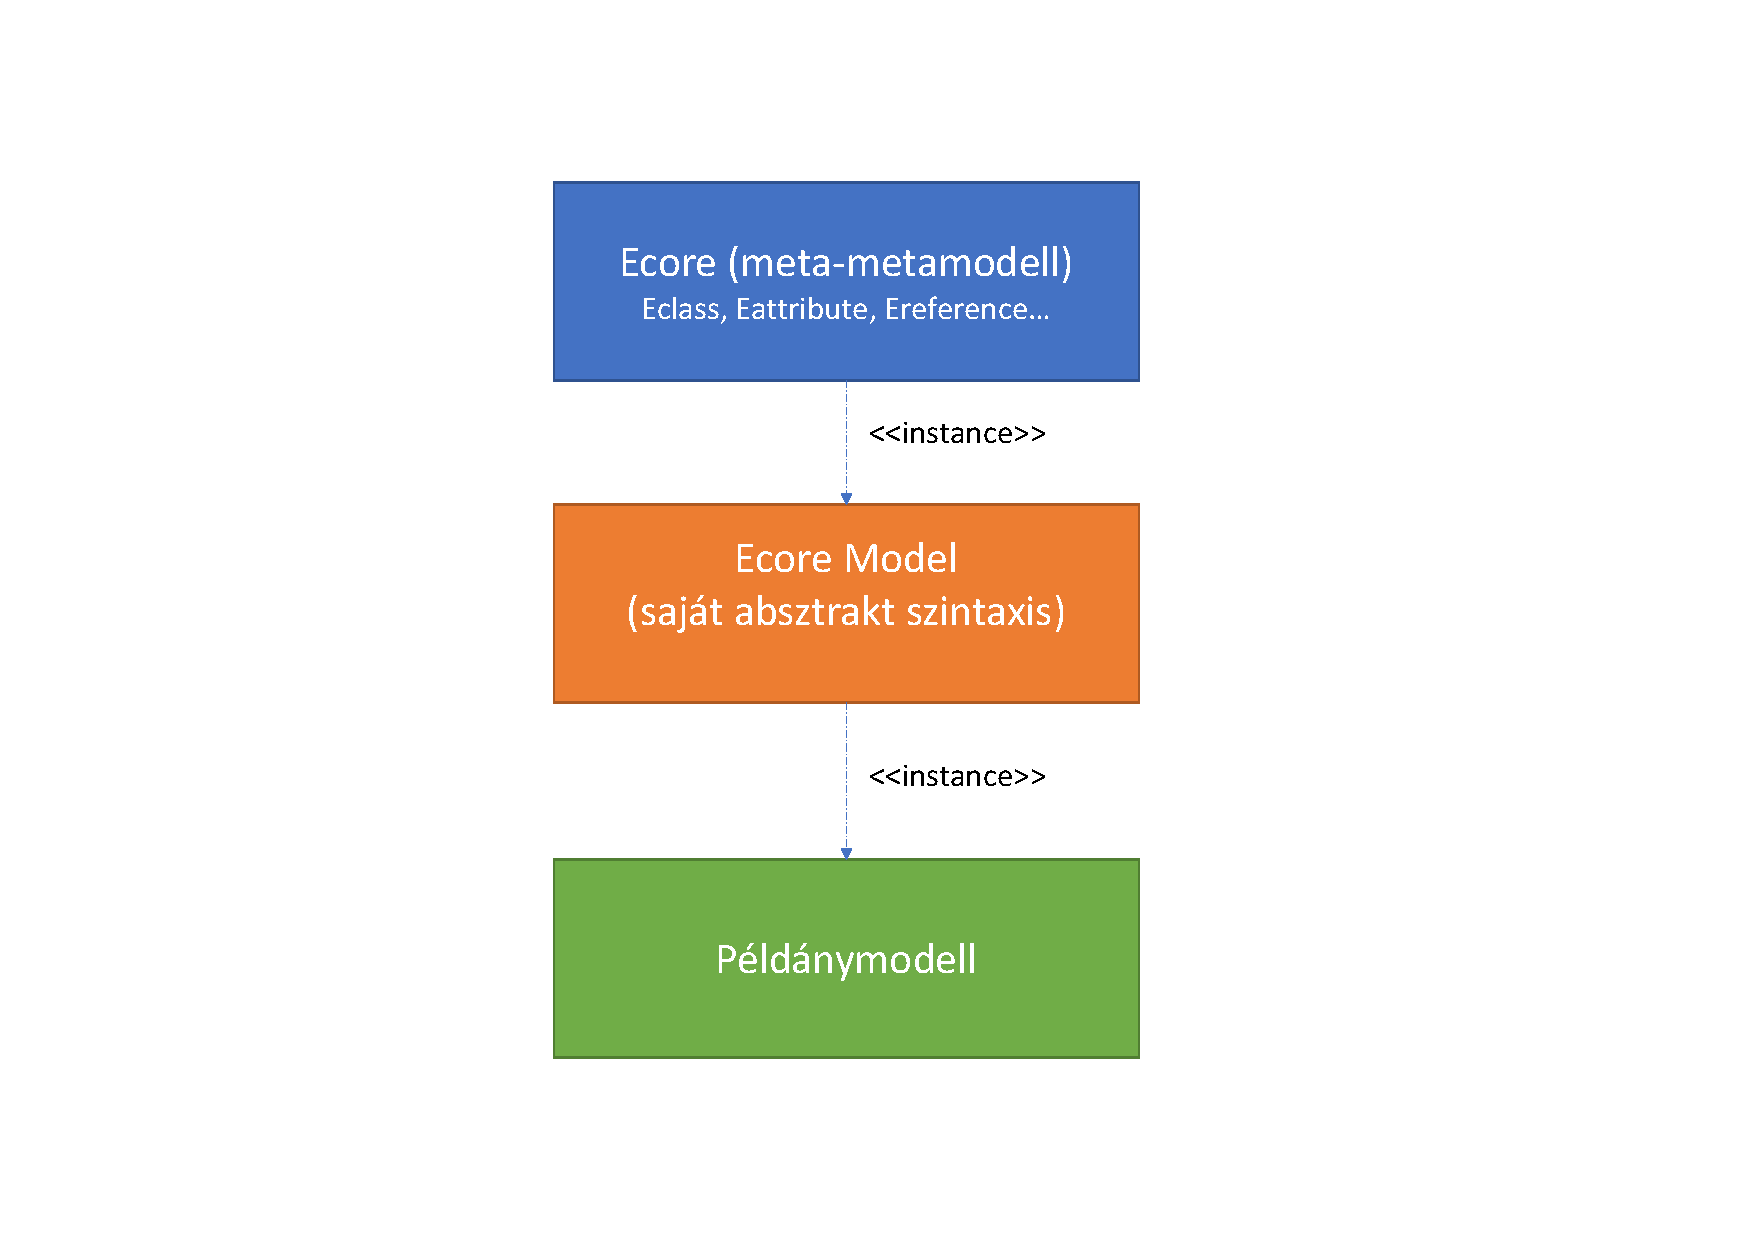
\includegraphics[width=100mm, keepaspectratio]{figures/ECore.pdf}
 	\caption{EMF meta szintek}
 	\label{fig:concept}
 \end{figure}
 

\section{Modell transzformációk}

Modellek származtatása más modellekből egy sokat alkalmazott megoldás a modell vezérelt fejlesztés során, hiszen így nem szükséges minden szakterület specifikus modellhez külön eszköz, ami ezekkel képes dolgozni. Ahhoz, ténylegesen származtatni tudjunk egy modellből egy másikat meg kell vizsgálni a szemantikájuk közötti kapcsolatokat és át kell hidalni a különbséget. Az ilyen jellegű szemantikai levezetést denotációs szemantikának nevezzük.

\begin{figure}[!ht]
	\centering
	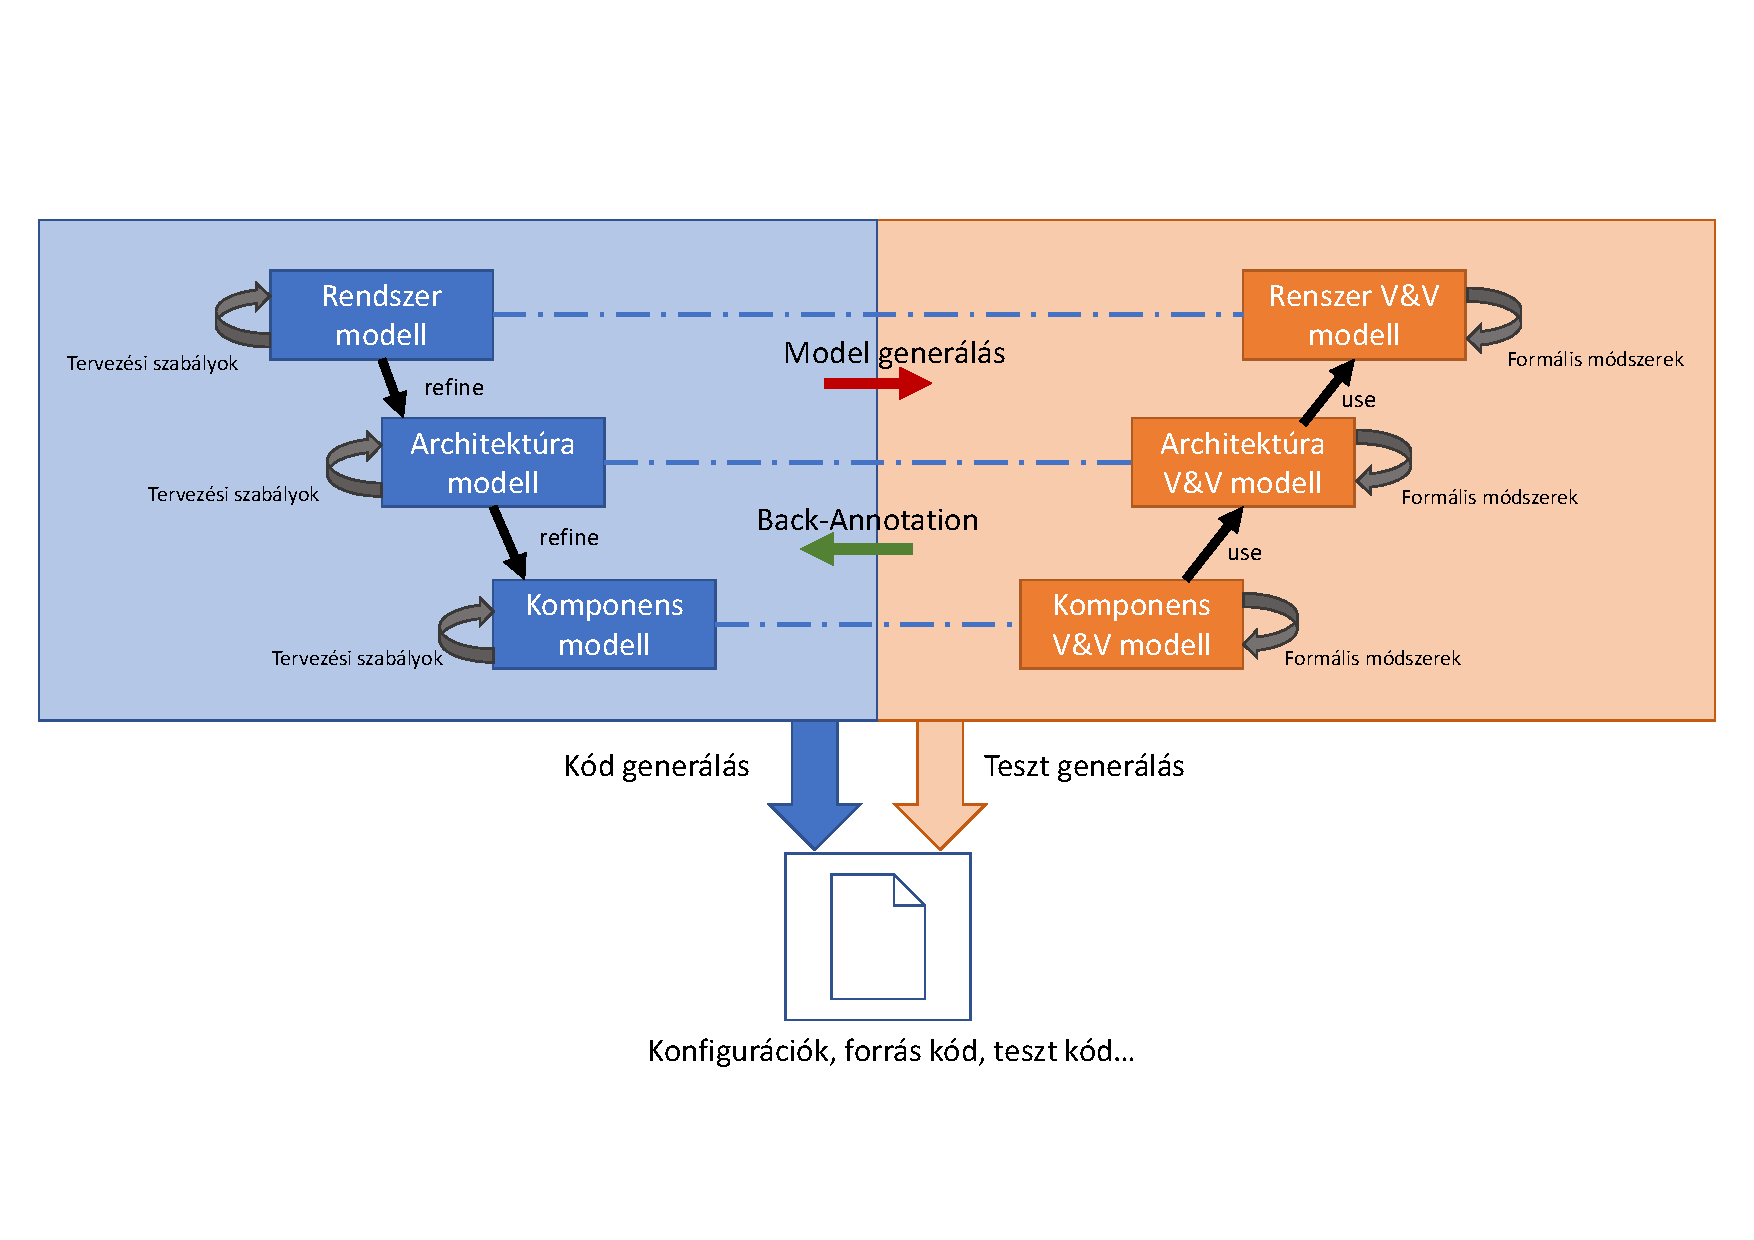
\includegraphics[width=100mm, keepaspectratio]{figures/Vmodel.pdf}
	\caption{Modell transzformációk alkalmazása a modell vezérelt fejlesztés során}
	\label{fig:concept}
\end{figure}

Modellek transzformálását sokféleképp végre lehet hajtani. Talán a legtriviálisabb megoldás a modell bejárása valamilyen általános célú programnyelv segítségével és a modell elemeinek egyenkénti feldolgozása. Ez a megoldás egyes esetekben elégséges lehet azonban nagyon nehéz karban tartani. Sokkal jobb megközelítés, hogy valamilyen lekérdező nyelvet alkalmazunk a modell bejárására. Ezek használata a programozó szemszögéből sokkal egyszerűbbek, hiszen deklaratív módon tudjuk megadni a lekérdezés specifikációját, ráadásul a lekérdezéseket különböző lekérdező motorok sokszor ki is optimalizálják, így egyes esetekben még hatékonyabb is lehet mint egy általános programozási nyelvvel történő keresések.

A VIATRA egy olyan technológia amivel modell lekérdezéseket és transzformációkat definiálhatunk. A lekérdezéseket egy speciális nyelv a Viatra Query Language (VQL) segítségével lehet leírni. Ez egy deklaratív nyelv amivel le tudjuk írni, hogy egyes elemek között milyen kapcsolatokat várunk.

\begin{lstlisting}[language=bash,frame=single,float=!ht]
pattern TranisitonsInStateMachine(stateMachine: StateMachine, transition: Transition){
	find RegionsInStatemachine(stateMachine, region);
	Region.transition(region, transition);
}
\end{lstlisting}

A VIATRA-val történő transzformációk két részből állnak: egy VQL nyelven leírt lekérdezés és egy imperatív módon leírt akció, ami minden illeszkedésre végrehajtódik.

\begin{lstlisting}[language=bash,frame=single,float=!ht]
	val transitionRule = createRule(transitionsInStateMachine).action[match | 
		//...
	].build
	
	//...
	
	def execute(){
		transitionRule.fireAllCurrent
	}
\end{lstlisting}

VIATRA-val kétféle transzformáció hozható létre. Batch transformation ami a programozó hívására elvégzi a transzformációt. Újbóli meghívás esetén a transzformációk ismét előröl végrehajtódnak. Illetve live transformation, ami figyeli a modellben történő változásokat (elemek törlése, létrehozása, frissítése) és ezeknek megfelelően hajt végre akciókat. Ennek során nem szükséges az egész modell leképzése, elég csak a változást érintő részek kezelése.


\section{MagicDraw pluginok}

A MagicDraw funkcionalításának bővítése pluginokkal lehetséges, ehhez a MagicDraw egy API-t biztosít melyet Open Api-nak neveznek ez lehetővé teszi, hogy hozzáférjünk a MagicDraw fő funkcióihoz. A plugin működéséhez két leíró fájlt kell előállítani. Az egyik a pluginDescriptor.xml ami a plugin telepítéséről és egyéb tulajdonságairól (vendor, név, verzió) tartalmaz információkat. Ez nem feltétlen szükséges a plugin futtatásához. A másik a plugin.xml ami nélkül a plugin nem fog betöltődni. Ez definiálja a plugin belépési pontját és a plugin classloaderjét. Az osztályok betöltéséhez a MagicDraw alapértelmezetten egy közös classpath-t használ, amin minden plugin osztozik. Ezt a plugin.xml-ben módosítani lehet, ha valamiért külön classloaderre lenne szükségünk a pluginunkhoz.

\paragraph{Példa:} plugin.xml tartalma
\begin{lstlisting}[language=bash,frame=single,float=!ht]
<plugin
id="magicdraw2gamma"
name="MagicDraw2Gamma Plugin"
internalVersion="1549381332"
version="1.0.0"
provider-name="BME-FTSRG"
class-lookup="LocalFirst"
ownClassloader="true"
class="hu.bme.mit.magicdraw2gamma.plugin.MagicDraw2GammaPlugin">

<requires>
	<required-plugin id="com.incquerylabs.v4md" name="V4MD" version="2.0.1" internalVersion="200003"/>
</requires>
<runtime></runtime>
</plugin>
\end{lstlisting}


A plugin.xml-ben hivatkozott osztálynak le kell öröklődnie a MagicDraw Plugin osztályából. A MagicDraw induláskor bejárja a plugins könyvtárát és beolvassa a plugin.xml-eket majd példányosítja és elindítja a ezeket, (meghívja az initet).

\begin{lstlisting}[language=bash,frame=single, float=t]

public class MyPlugin extends Plugin {

	@Override
	public void init() {
		//plugin started
	}

}
\end{lstlisting}

Az init során van lehetőségünk saját UI elemeink, működésünk hozzáadására a MagicDraw-hoz.

MagicDrawban ahhoz, hogy a modell elemekhez hozzáférjünk egy Session-t kell nyitni, ehhez a Sessionk manager osztály használható.

\begin{lstlisting}
	SessionManager.getInstance().startSession()
	...
\end{lstlisting}


\subsection{VIATRA használata MagicDrawban}

VIATRA használatára a MagicDrawban is lehetőségünk van. Ehhez egy open source plugint a V4MD-t érdemes használnunk. A plugin minden projekt megnyitásakor készít egy motort amivel lekérdezéseket és transzformációkat tudunk regisztrálni.

A motort a ViatraQueryAdapter osztály segítségével tudjuk elkérni vagy ha még nem létezett létrehozni.

\begin{lstlisting}
	ViatraQueryAdapter.getOrCreateEngine(project)
\end{lstlisting}



\chapter{MagicDrawToGamma}

A MagicDrawToGamma egy MagicDrawhoz készített állapottérkép verifikációs eszköz, amely formális módszerek segítségével képes ellenőrizni, hogy a rendszer teljesíti-e a felhasználók által megfogalmazott tulajdonságokat.

\section{Plugin működése}

A plugin legfőbb feladata SysML állapottérképek letranszformálása olyan modellekké, melyekhez a formális verifikáció elvégzése már támogatva van, persze mindezt a szemantika megtartása mellett. A Gamma Statechart Composition framework állapottérképek modellezését teszi lehetővé egy saját maga által definiált DSL segítségével. A Gamma képes a modellekből egy olyan .xml alapú dokumentumot generálni amit az UPPAAL nevű eszköz képes feldogozni és az ezek által leírt UPPAAL modelleken formális verifikációt végrehajtani. Az eredményt, azaz az ellenpéldákat, ha vannak, a Gamma képes feldolgozni és visszavezetni a Gamma modellekbe, ezt back-annotationnak nevezik.

A plugin a verifikáció első lépéseként a SysML állapottérképeket Gamma állapottérképekké alakítja, majd a Gamma funkcionalitását kihasználva létrehozza azokat az .xml formátomú dokumentumkat, melyeket az UPPAAL képes feldolgozni. Ezeket az ellenőrizendő tulajdonságokkal együtt az UPPAAL beolvassa és elvégzi a formális verifikációt, aminek eredménye (teljesültek a követelmények vagy sem) megjelenítésre kerülnek.

\begin{figure}[!ht]
	\centering
	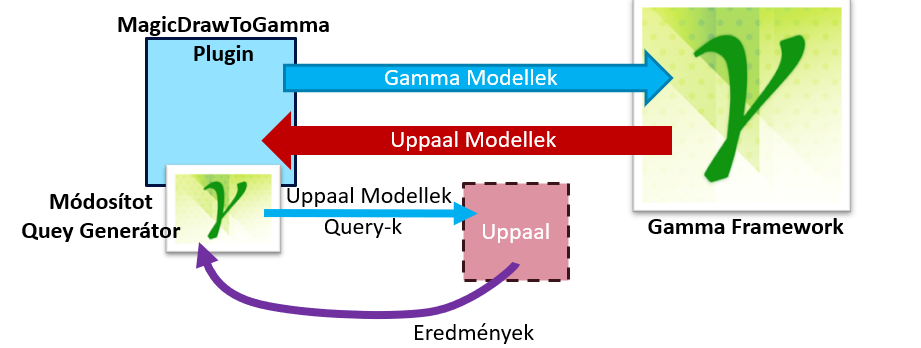
\includegraphics[width=100mm, keepaspectratio]{figures/concept.png}
	\caption{A plugin működése}
	\label{fig:concept}
\end{figure}

A plugin egyenlőre a back-annotationból származó információkat nem képes megjeleníteni, és csak single component állapottérképek transzformációjára képes.








\chapter{A plugin továbbfejlesztése}

\section{Kompozíció modellezése}
Állapottérképekkel rendszerek állapot és esemény alapú működését szoktuk leírni, legtöbbször azonban ezeket nem önmagukban hanem más modellek részeiként szoktuk használni, alacsonyabb szintű komponensek leírására, majd ezeket használva magasabb szintű komponenseket hozunk létre. A komponensek közti adatáramlások szintén fontos aspektusai egy rendszernek.


A Gamma keretrendszer egyik legkiemelkedőbb funkciója, hogy nem egyszerűen állapottérképek modellezésére ad lehetőséget, hanem ezek dekomponálására is. Az elemi komponens az állapotgép, ezeket felhasználva és a közöttük történő kommunikációk modellezésének segítségével összetett rendszereket vagyunk képesek leírni.

SysML-ben a rendszer funkcionális dekompozícióját Block Diagrammok segítségével végezzük, a komponensek kapcsolatát pedig Internal Block Diagrammokon tudjuk leírni.

\subsection{Szinktaktikai és szemantikai különbségek}

A két nyelv nagyon hasonlóan közelíti meg a rendszer dekomponálását. SysMLben blockokat azaz funkcionális egységeket definiáljuk és ezeket tartalmazási hierarchiába rendezzük magasabb szintű blokkokat definiálva, vagy ha top-bottom megközelítésben dolgozunk egy magasabb szintű blokkot bontunk fel részekre és a részeket még tovább kifejtük amennyire szükséges.

\begin{figure}[!ht]
	\centering
	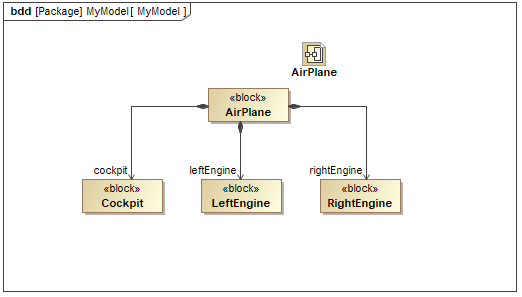
\includegraphics[width=75mm]{figures/examplebdd.png}
	\caption{Block Definition Diagram MagicDrawban}
\end{figure}

Ezt követően finomítjuk a modellt és a részek közötti kapcsolatokat is leírjuk. Ehhez portokat és konnektorokat használunk.
 
 \begin{figure}[!ht]
	\centering
	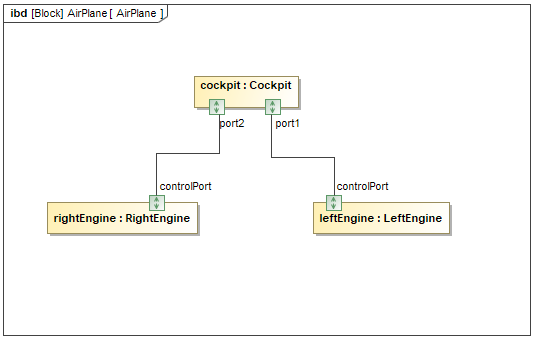
\includegraphics[width=75mm]{figures/exampleibd.png}
	\caption{Internal Block Diagram MagicDrawban}
\end{figure}

A Gammában a komponenseket és a kapcsolatokat köztük szöveges szintaxissal tudjuk leírni.

\begin{lstlisting}[language=bash,frame=single,float=!ht]
sync AirPlane [] {
	// Components of the composite model
	component leftEngine : LeftEngine
	component rightEngine : RightEngine

	// Connecting ports of components using channels
	channel [controller.PriorityControl] -o)- [prior.Control]
	channel [controller.SecondaryControl] -o)- [secondary.Control]

	channel [controller.PriorityPolice] -o)- [prior.PoliceInterrupt]
	channel [controller.SecondaryPolice] -o)- [secondary.PoliceInterrupt]
}
\end{lstlisting}


A Gamma megkülönbözteti a komponenseket aszerint, hogy ezek sorosan, vagy párhuzamosan működnek.
\subsection{Szinkron komponensek Gammában}
A Synchronous Component-ek olyan rendszereket reprezentálnak, melyek kommunikációja szinkron zajlik. A Gammában három féle elem van ami szinkron kommunikációt használ: StatechartDefinition, Synchronous Component, Cascade Synchronous Component. A komponensek szignálokkal kommunikálnak. Végrehajtás során a komponensek feldolgozzák a bejövő szignálokat és kimenő szignálokat állítanak elő, illetve megváltoztatják belső állapotukat.

\paragraph{Synchronous Composite Component:} a birtokolt komponensek végrehajtása ciklikusan történik, fixen meghatározott sorrendben, ami nem változik két végrehajtási ciklus között. A komponensek egy cikluson belül nem hatnak ki egymásra, az általuk küldött szignálok a következő ciklusban kerülnek feldolgozásra.

\paragraph{Cascade Composite Component:} ugyan azokat az elemeket tartalmazhatja, mint a Synchronous Composite Component, azonban komponensek által kibocsátott szignálok ugyan abban a végrehajtási ciklusban kerülnek feldolgozásra, fogadásra. Cascade komponensek esetében egy jólformáltsági kényszer, hogy komponensek közötti kommunikáció kör mentes legyen.

\subsection{Aszinkron komponensek Gammában}
Aszinkron komponensek olyan rendszereket reprezentálnak, ahol a komponensek egymástól független futnak. Az ilyen komponensek esetében a futási idő nem meghatározott. Aszinkron komponensek portokon keresztül kommunikálnak és pufferelt üzeneteket küldenek egymásnak. A Gammában kétféle aszinkron komponens van: Asynchronous Composite Component, Synchronous Component Wrappe

\paragraph{Asynchronous Composite Component:} Ugyan azokat az elemeket tartalmazzák, mint a Synchronous Composite Component, azonban aszinkron elemek nem tartalmazhatnak szinkron elemeket, így a szinkron működésű komponenseket be kell csomagolni egy Synchronous Component Wrapper-be.

\paragraph{Synchronous Component Wrapper:} Kompozit komponensek becsomagolására szolgál ezáltal aszinkron szemantikát adva neki. A Wrapper implicit rendelkezik a becsomagolt komponens portjaival, továbbá tartalmaz egy üzenet sort, ami tárolja a fogadott üzeneteket. Az üzenet sornak meghatározható a mérete, a fogadható üzenetek típusai és ezek az ezek közti prioritások.


\subsection{Gamma profil MagicDraw-hoz}

A Gamma szemantikájának MagicDraw-ban történő alkalmazását UML profiling segítségével érdemes megvalósítani. Ehhez sztereotípiákat kell definiálni amelyeket alkalmazni lehet SysML és UML modell elemeken, ezzel jelezve, hogy ezekre a Gamma által definiált szemantika az értelmezendő.

A Gamma MagicDraw profil SysML modellekhez készült. Mivel a SysML maga is egy sztereotípiákat definiáló profil a Gamma profil elemei a blokk sztereotípiából származnak le.

TODO: profil ismertetése

\section{Opaque kifejezések}

UML-ben és SysML-ben lehetőségünk van egyes elemek szöveges leírására is. A szöveges definíciókat tartalmazó eleket Opaque Expression-öknek nevezzük.

A MagicDraw nem írja elő,hogy milyen nyelvtant kell alkalmazni őrfeltételek vagy Opaque Expression formájában megadott akciókhoz, bár specifikálhatóvá tesz néhányat a felhasználónak (java, C, OCL).

Éppen ezért a kötetlenség miatt a MagicDrawToGamma a Gammában is használatos nyelvtant használta az őrfeltételek értelmezéséhez. Ez jelentősen megkönnyítette a modellek feldolgozását hiszen ezeket a kifejezéseket nem kellett Gamma kifejezésekké transzformálni.

Ahhoz, hogy a plugin szélesebb rétegek szémára is használható legyen érdemes lenne egy olyan nyelvet használni, amit gyakran alkalmaznak SysML modellek esetében.

\section{Object Contraint Language}

Az Object Constraint Language (OCL) egy deklaratív szabály leíró nyelv amit elsősorban jólformáltsági kényszerek leírására használnak, de állapottérképek őrfeltételeiként is alkalmazhatóak.

Ennek a nyelvnek a használatát az is ösztönzi, hogy ez része az UML szabványnak, így az UML alapú modelleken (pl. SysML-en is) szabvány szerint alkalmazható.

\subsection{OCL kifejezések alkalmazása}

OCL kifejezések alkalmazhatók:

\begin{itemize}
	\item Osztályok és típusok invariánsaként egy metamodellben
	\item Sztereotípiák típusainak invariánsaiként
	\item Viselkedések pre- és postkondícióihoz
	\item \textbf{Őrfeltételek leírására}
	\item jólformáltsági kényszerekhez
	\item modell lekérdezésekhez
\end{itemize}

\paragraph{Példa:} A Person osztály példányaiban az 'age' attribútum értéke nem lehet negatív.

\begin{lstlisting}[language=OCL,frame=single]
	context Person inv: self.age >=0
\end{lstlisting}

\paragraph{Példa:}  Meeting osztály do metódusa akkor hívható meg, ha 'canDo' értéke igaz
\begin{lstlisting}[language=OCL,frame=single]
context Meeting::do()
pre: self.canDo = true
\end{lstlisting}

Őrfeltételekként való alkalmazásnál a kontextus az állapotátmenet kell, hogy legyen. A self pointer pedig az állapottérképre, illetve ennek típusára mutat.

\subsection{Eclipse OCL}

OCL kifejezések EMF-re parsolásához az Eclipse-nek létezik egy implementációja ami képes bármilyen metamodellből parsert példányosítani és EMF alapú modellt generálnia kifejezésekből.



%\include{content/latex-tools}
%\include{content/thesis-format}
%\chapter{Összefoglalás}
\label{chap:osszefoglalas}
Dolgozatomban a feladatnak megfelelően bemutattam az állapottérképek formalizmusát és megterveztem egy folyamatot melynek segítségével támogatni lehet ezek formális verifikációját a MagicDraw modellező eszközben. A tervezett eszköz prototípusát megvalósítottam egy plug-in formájában melynek a működését egy esettanulmányon demonstráltam, végül pedig értékeltem az elvégzett munkát és megvizsgáltam a továbbfejlesztési lehetőségeket.

\paragraph{Az elvégzett munka fontosabb kontribúciói:}
\begin{itemize}
	\item Megfeleltetések megtervezése
	\begin{itemize}
		\item Összevetettem a két eszköz Metamodelljét
		\item Kiválasztottam az egymásnak megfeleltethető elemeket
		\item Odafigyeltem a szemantikai különbségekre
	\end{itemize}
	\item Leképzés implementációja
		\begin{itemize}
		\item modell transzformációkra specializált technológiát használtam
		\item az eszközt MagicDraw plug-in formájában valósítottam meg
	\end{itemize}
	\item Fejlesztőkörnyezet kialakítása
		\begin{itemize}
			\item összegyűjtöttem a szükséges dependenciákat
			\item odafigyeltem a tranzitív dependenciák helyes menedzselésére
		\end{itemize}
	\item Lehetővé tettem, hogy a MagicDraw-n belül elvégezhető legyen a verifikáció
			\begin{itemize}
			\item átvettem és módosítottam a Gamma Query Generátor funkcióját
		\end{itemize}

	\item Elméleti megközelítésből értékeltem a munkám
		\begin{itemize}
			\item esettanulmányon mutatom be az elkészült eszközt
			\item áttekintetem az alternatív megvalósítási lehetőségeket
		\end{itemize}	
\end{itemize}
Munkám eredményéül létrejött egy olyan MagicDraw plug-in amivel lehetőség nyílik állapottérképek formális verifikációjának végrehajtásába.

\section{Jövőben elvégzendő munka}

Az eddigi munkám során létrejött eszköz továbbfejleszthető, hogy lehetővé tegye komponens alapú modellek verifikációját is. A jövőben a leképzéseket kiterjesztem, hogy ezeket a modelleket is Gamma modellé lehessen transzformálni és elvégezni a formális verifikációt a rendszeren. Továbbá megtervezek egy olyan új funkciót ami megjeleníti a felhasználóknak azokat az utakat, amik a megszorításaik megsértéséhez vezettek. A felhasználói élmény javítása érdekében validációs szabályokat hozok létre, amik futásidőben figyelmeztetik a felhasználókat azoknak az elemeknek a használatára, amelyek felhasználása nem teszi lehetővé a leképzést, vagy a formális verifikáció végrehajtását. Továbbá megfontolom olyan elemek támogathatóságát, amik az állapottérképek újrahasznosítását teszik lehetővé (\emph{SubmachineState}).


%tervezett


% Acknowledgements
%~~~~~~~~~~~~~~~~~~~~~~~~~~~~~~~~~~~~~~~~~~~~~~~~~~~~~~~~~~~~~~~~~~~~~~~~~~~~~~~~~~~~~~
%%----------------------------------------------------------------------------
\chapter*{\koszonetnyilvanitas}\addcontentsline{toc}{chapter}{\koszonetnyilvanitas}
%----------------------------------------------------------------------------

Szeretnék köszönetet mondani mindazoknak a feladat elvégzése során segítették a munkám: Farkas Rebekának, aki konzulensemként mindig segítőkész, pozitív hozzáállásával, és szakmai tanácsival, kritikáival segítette a dolgozat létrejöttét. Továbbá Molnár Vincének aki a Gamma Statechart Composition Framework használatát javasolta és ötleteket adott a megvalósítható funkciókra vonatkozóan. Köszönöm továbbá az IncQuery Labs-nak, hogy rendelkezésemre bocsátották a plug-in skeletonjukat, és a náluk töltött szakmai gyakorlatom során szerzett gyakorlati tapasztalatokat, amik jelentősen megkönnyítették az implementáció elkészítését.


% List of Figures, Tables
%~~~~~~~~~~~~~~~~~~~~~~~~~~~~~~~~~~~~~~~~~~~~~~~~~~~~~~~~~~~~~~~~~~~~~~~~~~~~~~~~~~~~~~
%\listoffigures\addcontentsline{toc}{chapter}{\listfigurename}
%\listoftables\addcontentsline{toc}{chapter}{\listtablename}


% Bibliography
%~~~~~~~~~~~~~~~~~~~~~~~~~~~~~~~~~~~~~~~~~~~~~~~~~~~~~~~~~~~~~~~~~~~~~~~~~~~~~~~~~~~~~~
\addcontentsline{toc}{chapter}{\bibname}
%\bibliography{bib/mybib}


% Appendix
%~~~~~~~~~~~~~~~~~~~~~~~~~~~~~~~~~~~~~~~~~~~~~~~~~~~~~~~~~~~~~~~~~~~~~~~~~~~~~~~~~~~~~~
%%----------------------------------------------------------------------------
\appendix
%----------------------------------------------------------------------------
\chapter*{\fuggelek}\addcontentsline{toc}{chapter}{\fuggelek}
\setcounter{chapter}{\appendixnumber}
%\setcounter{equation}{0} % a fofejezet-szamlalo az angol ABC 6. betuje (F) lesz
\numberwithin{equation}{section}
\numberwithin{figure}{section}
\numberwithin{lstlisting}{section}
%\numberwithin{tabular}{section}

%----------------------------------------------------------------------------
%\section{A TeXstudio felülete}
%----------------------------------------------------------------------------
%\begin{figure}[!ht]
%\centering
%\includegraphics[width=150mm, keepaspectratio]{figures/TeXstudio.png}
%\caption{A TeXstudio \LaTeX-szerkesztő.} 
%\end{figure}


%\label{page:last}
\end{document}
